\documentclass[a4paper,12pt]{report}

\usepackage{../courslatex}
\usepackage{exos}
\usepackage{enumitem}

\setlist[enumerate]{align=left,leftmargin=1cm,itemsep=5pt,parsep=0pt,topsep=0pt,rightmargin=0.5cm}

\setlist[itemize]{align=left,labelsep=1em,leftmargin=*,itemsep=0pt,parsep=0pt,topsep=0pt,rightmargin=0cm}

\renewcommand{\titreChapitre}{Ch3\,: Calcul littéral} 
\renewcommand{\numeroSerie}{4}

\begin{document}
\vspace*{-2\baselineskip}
\textLigne{Activités}
\begin{acti}
	Les savants de la Grèce antique donnèrent des preuves géométriques des propriétés des nombres réels, basées sur l'aire du rectangle. 
	\begingroup
{%% do not forget to chage the default values inside a group
\belowdisplayskip=-10pt
	\begin{tasks}
	\task 	Pour illustrer la distributivité de la multiplication sur l'addition pour les nombres réels $a,b,$ et $c$, exprimer de deux manières l'aire du rectangle représenté ci-dessous\,:

	\begin{center}
	\begin{tikzpicture}
    \tkzDefPoint[label=below:{}](-1,-1){A}
    \tkzDefPoint[label=right:{}](-1,1){B}
    \tkzDefPoint[label=above:{}](2,1){C}
    \tkzDefPoint[label=above:{}](2,-1){D}
    \tkzDefPoint[label=above:{}](3,1){E}
    \tkzDefPoint[label=above:{}](3,-1){F}

    \tkzDrawPolygon(A,B,E,F)
    \tkzDrawSegment[dashed,dim={$b$,15pt,midway,font=\footnotesize}](B,C)
    \tkzDrawSegment[dashed,dim={$c$,15pt,midway,font=\footnotesize}](C,E)
    \tkzDrawSegment[dashed,dim={$a$,15pt,midway,font=\footnotesize}](A,B)
    \tkzDrawSegment[dashed](C,D)
	\end{tikzpicture}
\end{center}
	\task De manière semblables, illustrer géométriquement les identités suivantes\;:
	\[(a+b)^2 \quad \text{et}\quad (a+b)(c+d)\]
	\end{tasks}
}\endgroup
\end{acti}
\begin{acti}
En utilisant la lettre $n$ pour désigner un entier quelconque, exprimer sous forme littérale :
\begin{tasks}
\task trois entiers consécutifs;
\task le carré d'un entier impair quelconque;
\task un nombre positif, différence des carrés de deux nombres entiers consécutifs;
\task un multiple de 7;
\task un entier qui laisse un reste de 2 lorsqu'on le divise par 3 ;
\task un entier qui précède immédiatement un multiple de 4 ;
\task trois carrés parfaits consécutifs.
\end{tasks}
\end{acti}
\begin{acti}
Un rectangle possède une largeur de $a(>3) \mathrm{cm}$ et une longueur de $(a+4) \mathrm{cm}$. On lui enlève un carré de 3 cm de côté. Donner l'expression algébrique réduite de l'aire de la figure restante.
\end{acti}
\begin{acti}
	Pour chacune des expressions suivantes, préciser (sous : \enquote{Type}) s'il s'agit d'une somme ou d'un produit, et donner le nombre de termes (de cette somme ou de ce produit).
\begin{center}
	\begin{tabular}{|>{\stepcounter{rowcount}\alph{rowcount})}ll|l|l|}
    \cline{2-4}
    \multicolumn{1}{c|}{} & Expression& Type & Nombre de termes\\
   \noalign{\setcounter{rowcount}{0}} \hline
 & $4 \cdot x+1 \cdot(3 x-1) \cdot(5 x-1)+7 \cdot x$ & & \\
\hline&$-4 \cdot(x-y) \cdot(3 x-1) \cdot(5 x-1)$ & & \\
\hline&$(5 x-1) \cdot(5 x-1)+7(5 x-1)$ && \\
\hline&$(4 x-1)(3 x-4)(3 x+4)$ & &\\
\hline& $(4 x-1)(3 x-4)(3 x+4)-1$ & &\\
\hline&$((3 x-4)(3 x+4)-x+1) x$ & &\\
\hline& $(3 x-1)(x-1)+(4 x-1)(3 x-4)$ & &\\
\hline&$x^2-x^2(4x-1)(3x-4)x^2$& &\\
\hline
\end{tabular}
\end{center}
\end{acti}

\textLigne{Exercices}
\begin{exo}
Développer les produits suivants :
\begin{tasks}(4)
\task $7(8+9 x)$
\task $6 a\left(5 a^2-12 a\right)$
\task $-5(-7 y+11)$
\task $-12(-5 x-4)$
\task $-8\left(6 x^2+4 x-3\right)$
\task $-9 x^2\left(8 x^3+7 y\right)$
\task $7 a^5\left(6 a-4 a^2\right)$
\task $-5 x^4\left(7 x^4+9 x-1\right)$
\end{tasks}
\end{exo}
\begin{exo}
Développer les produits suivants :
\begin{tasks}(4)
\task $5(5+3 x)$
\task $2 x\left(2 x^2-2 x\right)$
\task $-5(-5 y+9)$
\task $-1(-3 x-3)$
\task $\left(x^2+x-1\right)(-1)$
\task $-2(x+y)$
\task $\left(1+x^2\right)\left(x^2-4\right)$
\task $-3 x^2\left(1-2 x^2+3 x\right)$
\task $(5+3 x)(x-1)$
\task $3 x y\left(x^2 y+x-1\right)$
\task $\left(4-x^2\right)\left(1-4 x^2\right)$
\task $\left(-4 x y^3-x^3 y\right)(-3 y)$
\task $-2(x+3)(x-1)$
\task $3(x-3)(x-3)$
\task $(-2 x+3)(x-1)$
\task $(-2 x+3)(3-2 x)$
\end{tasks}
\end{exo}
\begin{exo}
L'aire d'un rectangle est de $4 a^2+6 a$. Déterminer sa longueur, si la largeur mesure $2 a$.
\end{exo}
\begin{exo}
Développer et réduire le produit: $\left(n^2+n+1\right)\left(n^2-n+1\right)$. 
\begin{comment}
$\left(^*\right)$ Déterminer toutes les valeurs de l'entier naturel $n$, pour lesquelles $n^4+n^2+1$ est un nombre premier.
\end{comment}
\end{exo}
\begin{exo}
L'égalité suivante est-elle une identité : $\left(x^2+2 x+2\right)\left(x^2-2 x+2\right)=x^4+4$~?
\end{exo}

\begin{comment}
\begin{exo}
(*) Si $10 a+b$ est un multiple de $7, a-2 b$ est-il multiple de 7~?
\end{exo}
\end{comment}
\begin{exo}
Effectuer les produits suivants (résultat réduit).
\begin{tasks}(3)
\task $(2 y-3)(5+3 x)$
\task $(5+2 x)(2 x-3)$
\task $(3-y)(-5 y+9)$
\task $\left(x^2+x-1\right)(x-1)$
\task $(y-x)(x+y)$
\task $(x+1)(x-1)(x+2)$
\task $(2 x-1)(x+3)(1-x)$
\task $\left(1+x^2\right)\left(x^2-4 x+2\right)$
\task $(x+2)^3$
\task $\left(z^3-5 x^3 z+2 z\right)\left(z^3-3 x\right)$
\task $(2-x)\left(x^2+4\right)(2+x)$
\task $(x-1)^4$
\end{tasks}
\end{exo}


\begin{exo}
Réduire autant que possible (expression finale sans parenthèses).
\begin{tasks}(3)
\task $2 x-2 x$
\task $(2 x)(-2 x)$
\task $2(x-2) x$
\task $-5 y+9 y$
\task $-(5 y+9 y)$
\task $(-5 y)(+9 y)$
\task $(-5 y+9) y$
\task $(-5 y)+9 y$
\task $-5(y+9) y$
\task $-5(y+9 y)$
\task $-x(-x)(-1)$
\task $-x(-x-1)$
\task $-(x-x)-1$
\task $x \cdot x \cdot x+x \cdot x$
\task $x \cdot x \cdot(x+x) \cdot x$
\end{tasks}
\end{exo}
\begin{exo}
Un élève a développé tous les produits de trois des binômes $(x+1),(x-1),(x+2)$ et $(x-2)$, de toutes les manières possibles, sans répétition d'un binôme. Il a noté les résultats suivants :
$$
x^3-x^2-4 x+4, x^3-2 x^2-x+2, x^3+2 x^2-x-2 \text { et } x^3+x^2-4 x-4 \text {. }
$$
Malheureusement, cet élève ne se souvient pas dans quel ordre il a effectué ses calculs.
Comment peut-on l'aider à s'y retrouver immédiatement, par une simple observation~?
\end{exo}
\begin{exo}
	Développer les expressions de l'activité 4 aux lettres a), c), e), f), g) et h). 

(Expression réduite et ordonnée par puissances décroissantes.)
\end{exo}
\textLigne{Automatismes}

\begin{comment}
\begin{auto}
	Réduire.
\begin{tasks}(2)
\task $-(-2 x)-(-(-x+3 x))$
\task $4 a-(2 b-(-a+b)-b)$
\task $-5 x-(-3 y-(-x-(2 x-y)-y)+4 x)-y$
\task $-2 w-(3 w-2 t)-(-w-(3 w+t)+w)-2 t$
\task $2 a+5-(3 a+(5-(-2+2 a))+7 a)$
\task $-\left(-3 x^3+2-\left(7 x^3+4-\left(10-x^3\right)+3 x^3\right)+15\right)$
\end{tasks}
\end{auto}
\begin{auto}
	Réduire.
\begin{tasks}(2)
\task $3 a-((-2 a+5 a)-(-2 a))-a$
\task $-(-(-2 a+3 b)-4 a)-(-3 b)$
\task $(-5 x-y)-(3 x-((x-y)-(2 x+y))-x)$
\task $7 a^2-\left(-2 a^2-\left(-4 a^2-b\right)-5 b\right)-2 b$
\task $-(-(-(-7 a)-1)-1)-1$
\task $7 a^2 b-\left(-3 a^2 b-\left(2 a b^2+a^2 b-\left(-a b^2\right)\right)+2 a^2 b\right)$
\end{tasks}
\end{auto}
\begin{auto}
Développer et réduire.
\begin{tasks}(3)
\task $3 a^2 \cdot\left(2 a b+b^2\right)$
\task $\left(7 a b-3 a^2\right) \cdot 3 a b$
\task $2 a^3 \cdot(5 a-3 b)$
\task $\left(4 a^2 b-7 a b^2\right) \cdot a^3$
\task $4 x^2 \cdot\left(5 x y-x^2\right)$
\task $(3 a-2 b) \cdot 7 a b$
\end{tasks}
\end{auto}
\begin{auto}
Développer et réduire.
	\begin{tasks}(2)
\task $2 \cdot(3 x+5)-3 \cdot(2 x-4)$
\task $4 \cdot\left(2 a^2+b\right)+3 \cdot\left(4 a^2-b\right)$
\task $7 \cdot\left(x^4+2 y^4\right)-2 \cdot\left(2 x^4+y^4\right)$
\task $10 \cdot(3 a b-2 b c)-5 \cdot(2 a b+3 b c)$
\task $-4 \cdot(5 a-2 b)+4 \cdot(2 a-5 b)$
\task $2 \cdot(5 a-2 b+c)+3 \cdot(a-b+3 c)$
\end{tasks}
\end{auto}
\begin{auto}
Développer et réduire.
	\begin{tasks}(2)
\task $3 \cdot\left(x^2-5\right)-2 \cdot\left(x^2+7\right)$
\task $5 \cdot(2 x-y)+3 \cdot(2 x+3 y)$
\task $4 \cdot\left(a^3+2 b^3\right)-\left(2 a^3-b^3\right)$
\task $5 \cdot(3 x y-2 y)-4 \cdot(2 x y-3 y)$
\task $-4 \cdot\left(2 a^2 b-3 a c\right)+2 \cdot\left(3 a^2 b-2 a c\right)$
\task $3 \cdot\left(x^2-4 y^2-4\right)-\left(2 x^2+3 y^2-1\right) \cdot 4$
\end{tasks}
\end{auto}
\begin{auto}
Développer et réduire.
	\begin{tasks}(2)
\task $3 a^2 \cdot(2 a-b)-2 a^2 \cdot(4 a-3 b)$
\task $7 x y \cdot(2 x-3 x y)+3 x^2 \cdot\left(y^2-y\right)$
\task $2 z^2 \cdot(3 z-2 x)-4 z^2 \cdot(z-2 x)$
\task $5 a^2 b \cdot\left(a^2 b+4 b^2\right)-7 b^2 \cdot\left(2 a^4-a^2 b\right)$
\task $x^3 \cdot\left(2 y^2-3 x y\right)-2 x y^2 \cdot\left(5 x^2-4 x^3\right)$
\task $2 z \cdot w \cdot\left(z^2-z w+1\right)+3 z w \cdot\left(z^2-2 z w-1\right)$
\end{tasks}
\end{auto}
\begin{auto}
Réduire.
\begin{tasks}(3)
\task $\dfrac{4 x}{3}-\dfrac{5 x}{6}$
\task $\dfrac{2 x}{7}-\dfrac{x}{3}$
\task $\dfrac{2 x}{9}-\left(\dfrac{5 x}{6}+\dfrac{x}{4}\right)$
\task $\dfrac{3 x}{5}+x$
\task $\dfrac{3 x}{4}-\dfrac{2 x}{3}+\dfrac{x}{6}$
\task $\left(\dfrac{3 x}{5}-\dfrac{2 x}{3}\right)+\dfrac{x}{15}$
\end{tasks}
\end{auto}
\begin{auto}
Réduire.
	\begin{tasks}(3)
\task $\dfrac{x+4}{4}+\dfrac{x-3}{3}$
\task $\dfrac{x}{4}-\dfrac{x-2}{5}$
\task $\dfrac{2 x+1}{2}-\dfrac{2-3 x}{3}$
\task $\dfrac{x-1}{3}-\dfrac{2 x-3}{6}+\dfrac{2 x+1}{2}$
\task $\dfrac{x}{5}-\dfrac{2 x+1}{2}+\dfrac{5-4 x}{10}$
\task $\dfrac{2 x+2}{6}-\dfrac{12 x-4}{24}+\dfrac{6 x+9}{27}$
\end{tasks}
\end{auto}
\begin{auto}
Réduire.
\begin{tasks}(3)
\task $\dfrac{2 x-3}{3}+\dfrac{5-2 x}{5}$
\task $\dfrac{-2 x}{4}-2 x$
\task $\dfrac{4 x-2}{4}-\dfrac{1-2 x}{2}$
\task $\dfrac{3 x-8}{2}+\dfrac{3 x+10}{10}-\dfrac{5-x}{5}$
\task $\dfrac{x}{3}-\dfrac{3 x-1}{2}+\dfrac{11 x-3}{6}$
\task $\dfrac{4 x+8}{8}-\dfrac{6 x+9}{18}+\dfrac{15-5 x}{20}$
\end{tasks}
\end{auto}

\begin{exo}
(*) Voici deux propriétés $P_1$ et $P_2$. Choisir à chaque fois $P_1 \Rightarrow P_2, P_1 \Leftarrow P_2$ ou $P_1 \Leftrightarrow P_2$. Donner un contre-exemple pour les implications non retenues. (Démontrer les implications retenues~?)
\begin{tasks}(1)
\task Dans l'ensemble des entiers naturels :
$P_1: n$ est multiple de $2 ; \quad P_2: n$ est multiple de 4
\task Dans l'ensemble des nombres entiers :
$P_1:$ le carré de $n$ est impair; $\quad P_2: n$ est impair
\task Dans l'ensemble des nombres entiers $n$ plus grands que 2 :
$P_1: n$ est de la forme $4 k+1$ ou $4 k+3$, ( $k$ entier) ;
$P_2: n$ est un nombre premier
\end{tasks}
	\end{exo}
\begin{exo}
(*) On considère les propositions $A$ : " $n$ est un entier pair" et $B$ : " $n^2$ est un entier pair".
\begin{tasks}
\task Démontrer l'implication : $A \Rightarrow B$.
\task Démontrer l'implication réciproque : $B \Rightarrow A$.
\task donc écrire l'équivalence $A \Leftrightarrow B$ (c.-à-d. " $n$ est pair $\Leftrightarrow n^2$ est pair ").
\end{tasks}
\end{exo}
\end{comment}

\end{document}

